\chapter{Results}\label{ch:results}

As outlined in Chapter \ref{ch:method}, the Ensemble Kalman Filter is a data
assimilation method which aims to approximate the effect of the original Kalman
Filter by representing the state of the model on which it is operating as an
ensemble of state samples.
The aim of applying this ensemble method is to overcome the difficulties
encountered by the original Kalman Filter when being applied to non-linear
models, and when attempting to propagate the state covariance matrix for models
with high dimensionality.
This method has been applied to an agent based model of pedestrian movement
(documented in Section \ref{sec:method:model}) with a view to reducing the error
in the model with respect to the ground truth.
This Section will therefore aim to present the results of the preliminary
experiments undertaken.
This is be achieved by first showing the impact of the filtering process on the
overall model state, then focusing in on a single agent in the model.
Finally a comparison of the model error for before updating, after updating and
the observations used to update will be provided at each of the time-steps in
which assimilation takes place.
It should be noted that this section adopts the common terminology of
``forecast'' to mean the state predicted by the model before updating, and
``analysis'' to mean the state after updating.

\section{Impact of Ensemble Kalman Filter on model
state}\label{sec:results:model}

This section focuses on the impact of the Ensemble Kalman Filter on the model
state by showing the state of the model before and after the update process (at
$t=100$), along with the respective ground truth and associated synthetic
observations.
The model state shown in Figure \ref{fig:enkf_abm} is represented by the
ensemble mean position for each agent.

\begin{figure}[h]
    \centering
    \begin{subfigure}[h]{\textwidth}
        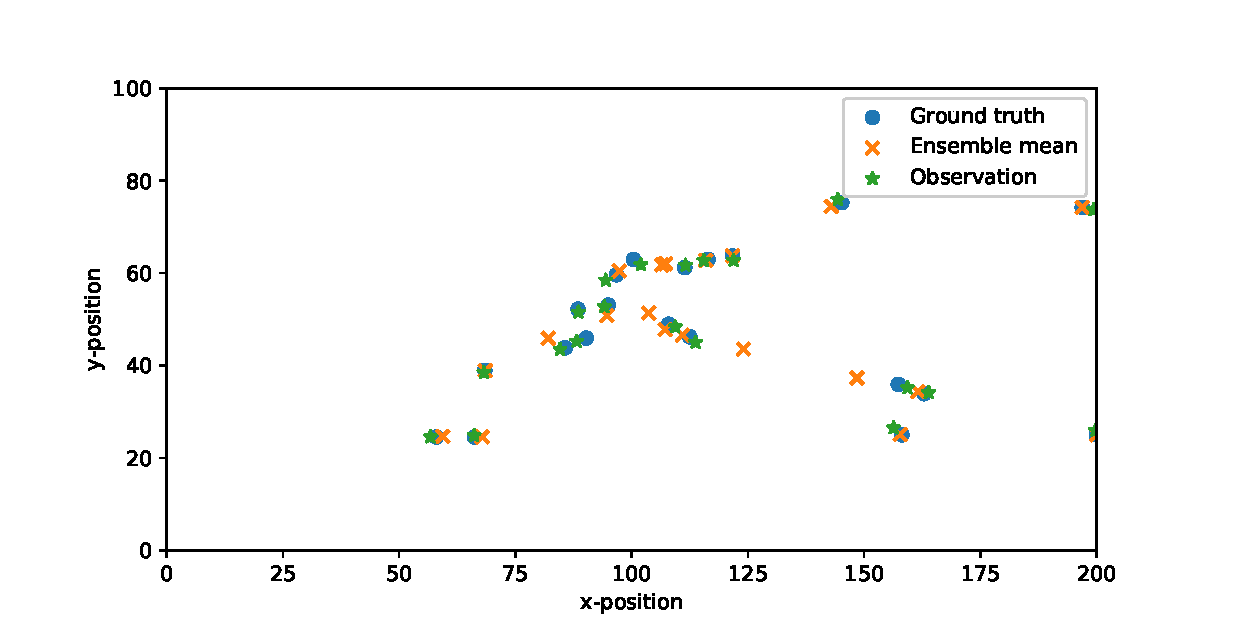
\includegraphics[width=\textwidth]{before_update_100.eps}
        \caption{Before update.}\label{fig:abm_before}
    \end{subfigure}

    \begin{subfigure}[h]{\textwidth}
        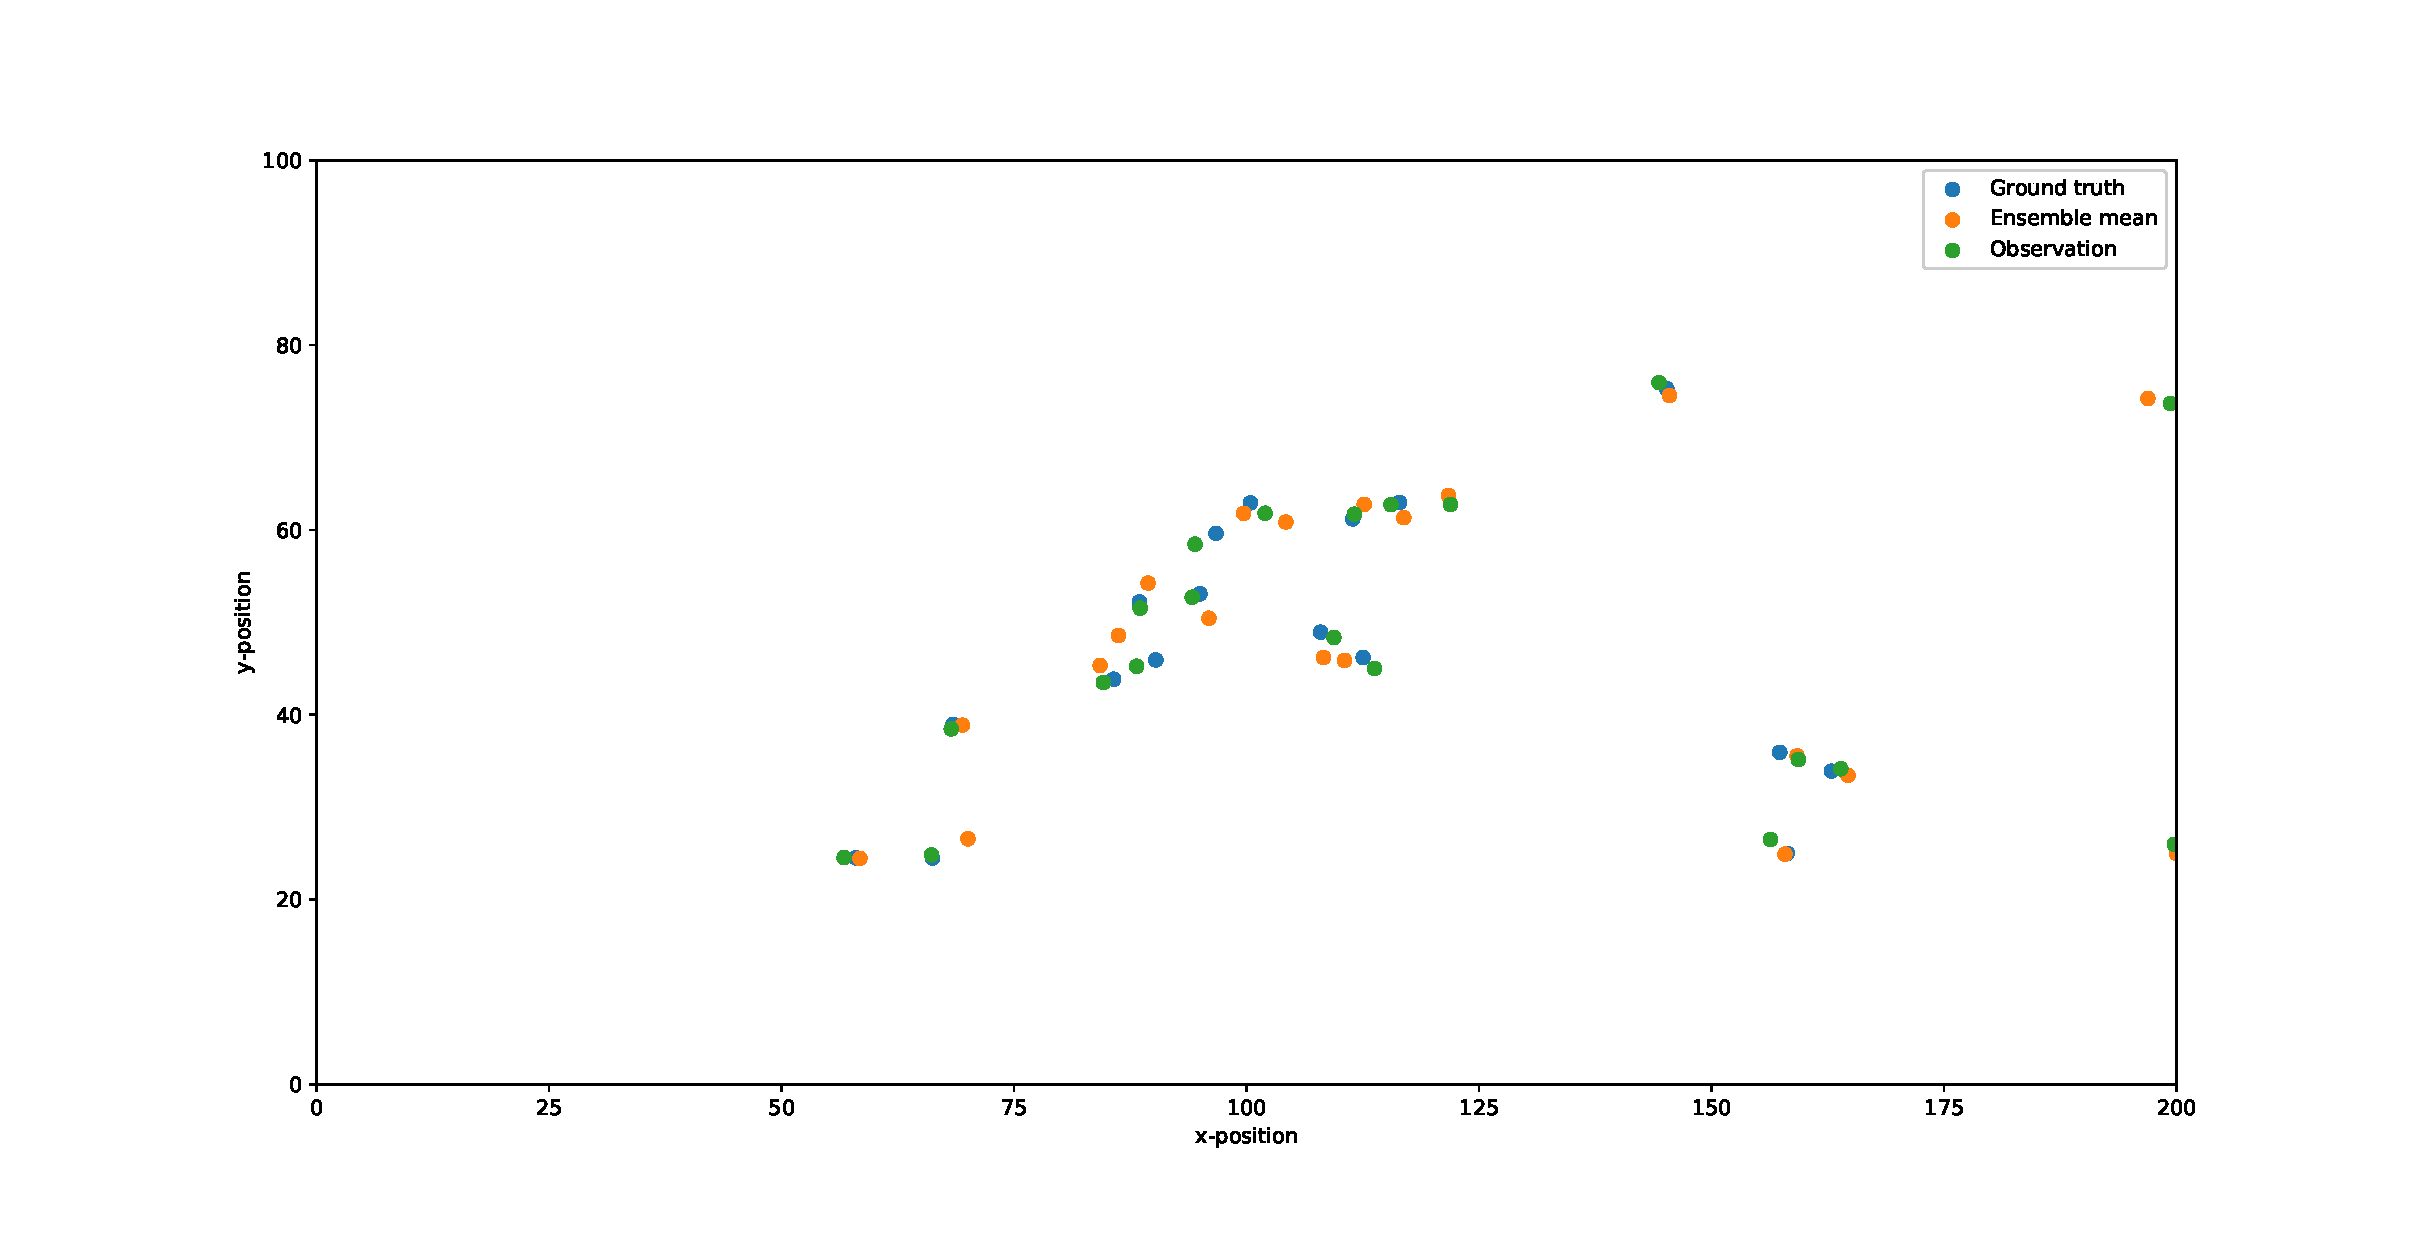
\includegraphics[width=\textwidth]{after_update_100.eps}
        \caption{After update.}\label{fig:abm_after}
    \end{subfigure}
    \caption[Effect of Ensemle Kalman Filter update on state of
    model.]{\centering Effect of Ensemble Kalman Filter update on state of
    agents in model ($k=100$).}\label{fig:enkf_abm}
\end{figure}

It can be seen that in the case of many agents, the forecast position is already
very close to both the ground truth and the respect observation of the agent.
This is a consequence of the design of the model --- when unimpeded, agents take
as direct a route as possible towards their target destination.
As a result, in these cases, the agent motion simulated by \texttt{base\_model}
and by the filter ensemble members is often the same.
This can be observed in agents that have advanced ahead of others and are close
to reaching their respective exits, and in slower agents that lag behind (Figure
\ref{fig:abm_before}).
Where the ensemble mean agent position forecast is already close to the ground
truth, the application data assimilation has little effect, as revealed by
comparing Figures \ref{fig:abm_before} and \ref{fig:abm_after} for the
aforementioned selections of agents.

In cases where agents interact, however, we observe that the ground truth and
ensemble mean forecast differ; this can be seen where agents crowd near the
centre of the environment in Figure \ref{fig:enkf_abm} (e.g. agents whose
forecast positions lie in the range $80<x<125, 40<y<55$).
In the case of these agents, the forecast ensemble mean agent positions lie
further away from the ground truth; indeed the forecast for some agents may lie
closer to the ground truth for different agent than the ground truth of the
original agent. 
In these cases, it can be seen by comparing Figures \ref{fig:abm_before} and
\ref{fig:abm_after} that the application of the Ensemble Kalman Filter is
effective in updating the ensemble mean state such that the analysis position of
the agents is closer to the ground truth.

\section{Impact of Ensemble Kalman Filter on agent
state}\label{sec:results:agent}

Whilst the previous section sought to show the efficacy of the Ensemble Kalman
Filter in updating the model state to reduce the error with respect to the
ground truth, this section focuses in on the impact of the data assimilation
method on the state of one of the agents in the model.
In particular, this allows us to examine the effect of applying data
assimilation to the state of each of the ensemble members.

\begin{figure}[h]
    \centering
    \begin{subfigure}[h]{\textwidth}
        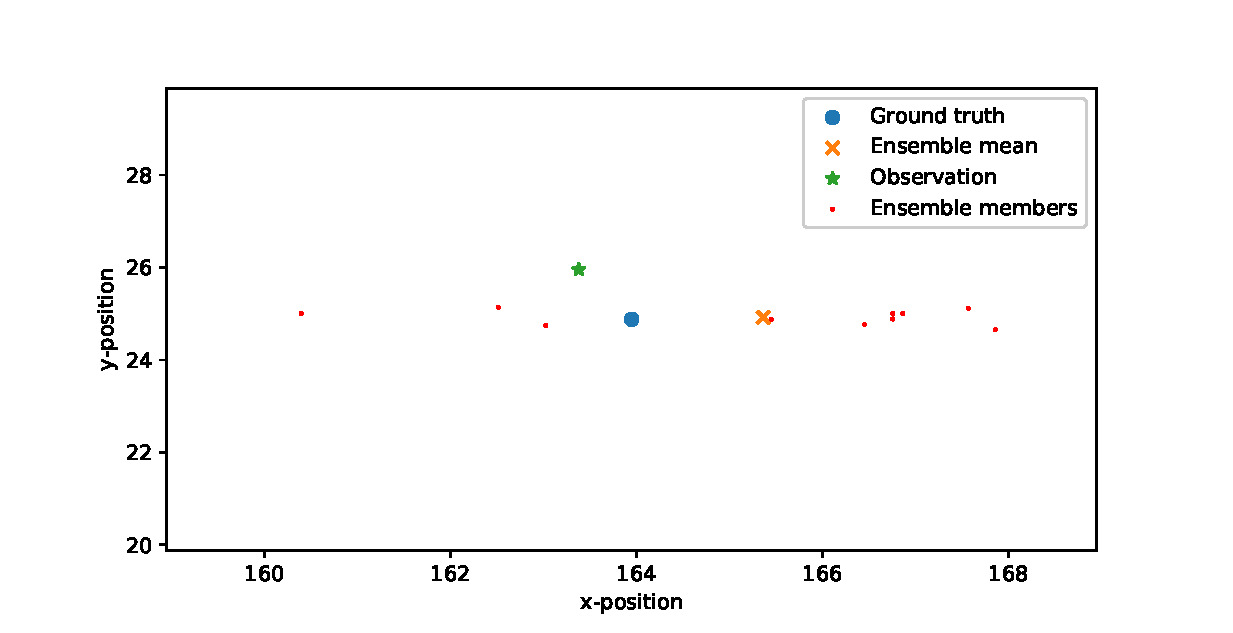
\includegraphics[width=\textwidth]{before_update_250_single.eps}
        \caption{Before update.}\label{fig:abm_before_single}
    \end{subfigure}

    \begin{subfigure}[h]{\textwidth}
        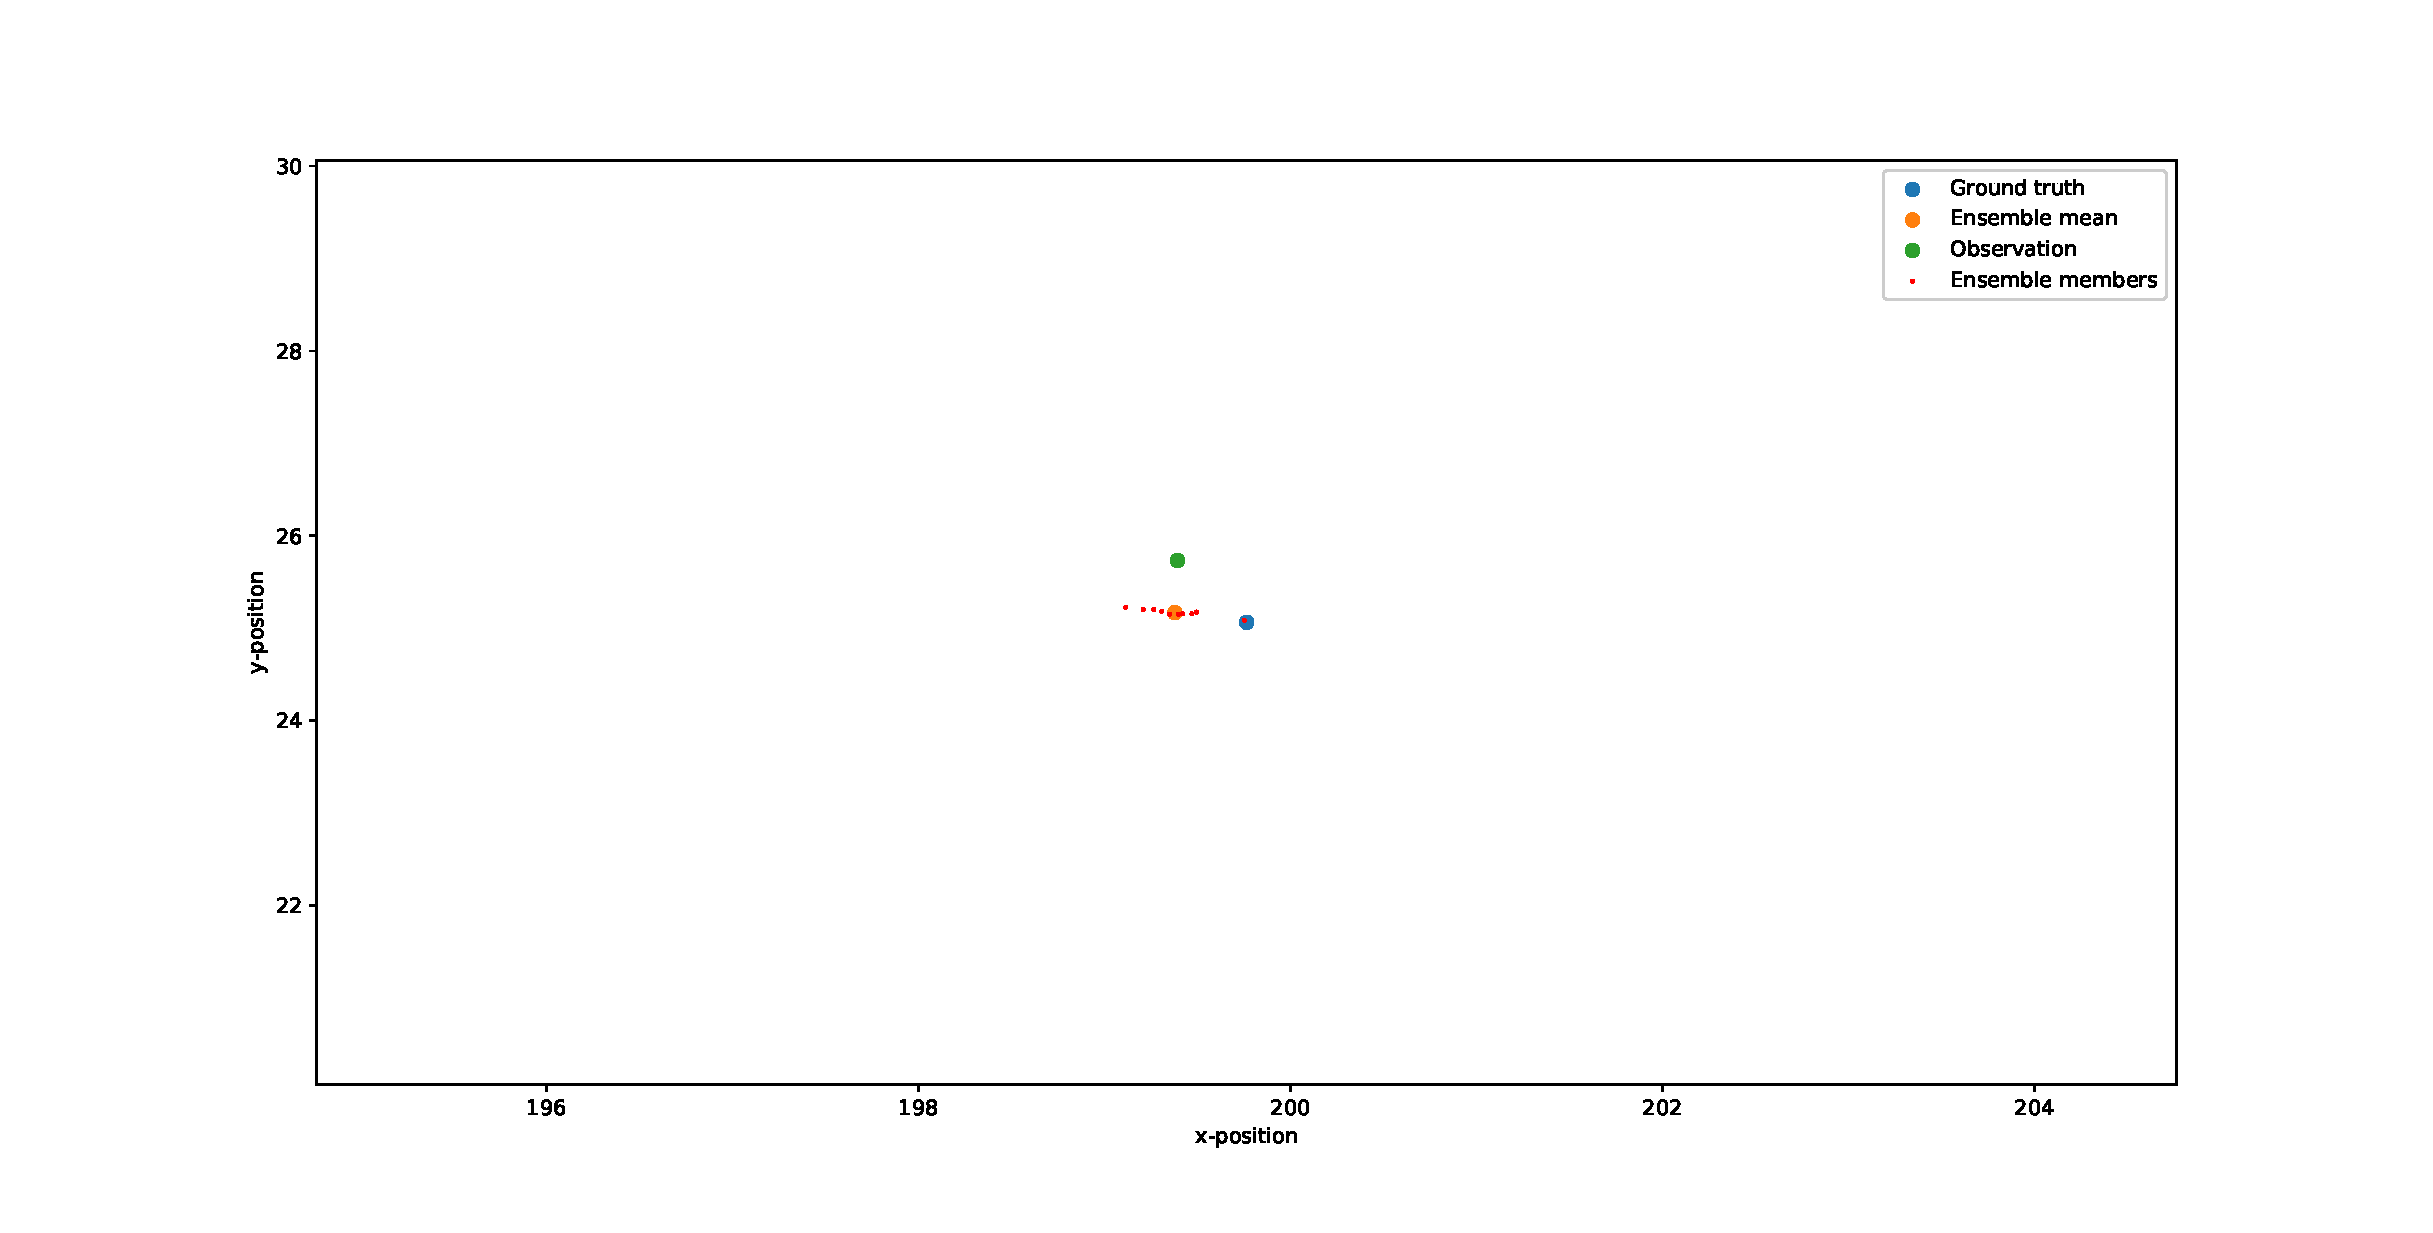
\includegraphics[width=\textwidth]{after_update_250_single.eps}
        \caption{After update.}\label{fig:abm_after_single}
    \end{subfigure}
    \caption[Effect of Ensemble Kalman Filter update on state of a single agent
    in the model.]{\centering Effect of Ensemble Kalman Filter update on state
    of ensemble members for a single agent in the model
    ($k=250$).}\label{fig:enkf_abm_single}
\end{figure}

In Figure \ref{fig:abm_before_single}, it can be seen that the error in the
forecast ensemble mean is only slightly worse than the observation error.
There is, however, large variation in the error of the members of the ensemble;
in the best case, one of the ensemble members exhibits error approximately equal
to the observation, but in the worst case, one of the ensemble members exhibits
error approximately four times that of the observation.
The forecast ensemble members appear to have diverged predominantly in the
$x$-direction, indicating that the dispersion is likely a result of the agent
getting stuck behind another in some of the ensemble realisations but not in
others.
Upon updating the model state based on the observation, the analysis ensemble
mean lies very close to the ground truth, greatly reducing the error in the
ensemble mean as seen in Figure \ref{fig:abm_after_single}.
The figure also shows that the error in the ensemble members falls as well, as
they converge on the ground truth.
This further confirms that the Ensemble Kalman Filter is effective in improving
the accuracy with which we can simulate pedestrian movement through agent-based
modelling.

\section{Comparison of errors in forecast, analysis and
observations}\label{sec:results:comparison}

Finally, we compare the error in the model forecasts, model analysis and
observations at each of the instances when data assimilation is undertaken (data
assimilation is undertaken every 50 time-steps).
The model forecast is taken to be the state produced by averaging the position
of each of the agents over the ensemble after undertaking the prediction
procedure, but before the update procedure; correspondingly, the model analysis
is taken to be the state produced by averaging the position of each of the
agents over the ensemble after having undertaken the update procedure.
The errors presented in Figure \ref{fig:rmse_comparison} are the root mean
squared error per agent at a given time-step $k$, where errors are taken in
euclidean distance between the true state and state given by the forecast,
analysis or observation:
\begin{equation}
    RMSE_{k}^{*} = \sqrt{\frac{1}{L} \sum_{j=0}^{L}
                    \left(
                    \| \mathbf{x}_{k}^{*} - \mathbf{x}_{k}^{t} \|_{2}
                    \right) ^ 2},
\end{equation}
where $L$ is the number of agents, $\mathbf{x}_{k}^t$ is the true agent position
at time-step $k$, $\mathbf{x}_{k}^{*}$ is the agent position for which we wish
to calculate the error at time-step $k$ (be it forecast position, analysis
position or observed position), and $\| * \|_2$ is the operator for calculating
the length of the contained vector known as the $2$-norm; for example,
$RMSE_{100}^{f}$ would represent the error in the forecast at $k=100$,
$RMSE_{200}^{a}$ would represent the error in the analysis at $k=200$, and
$RMSE_{300}^{o}$ would represent the error in the observations at $k=300$.
Figure \ref{fig:rmse_comparison} shows how the error for each of the forecast,
analysis and observation vary with each of the assimilation steps (for this
experiment, assimilation takes place every 50 time-steps).
The observations are produced by adding unbiased normally distributed random
noise with a standard deviation of $1$ to the true state, it is unsurprising to
observe that the error in the observations is consistently $1$ at each of the
assimilation steps.

\begin{figure}[h]
    \centering
    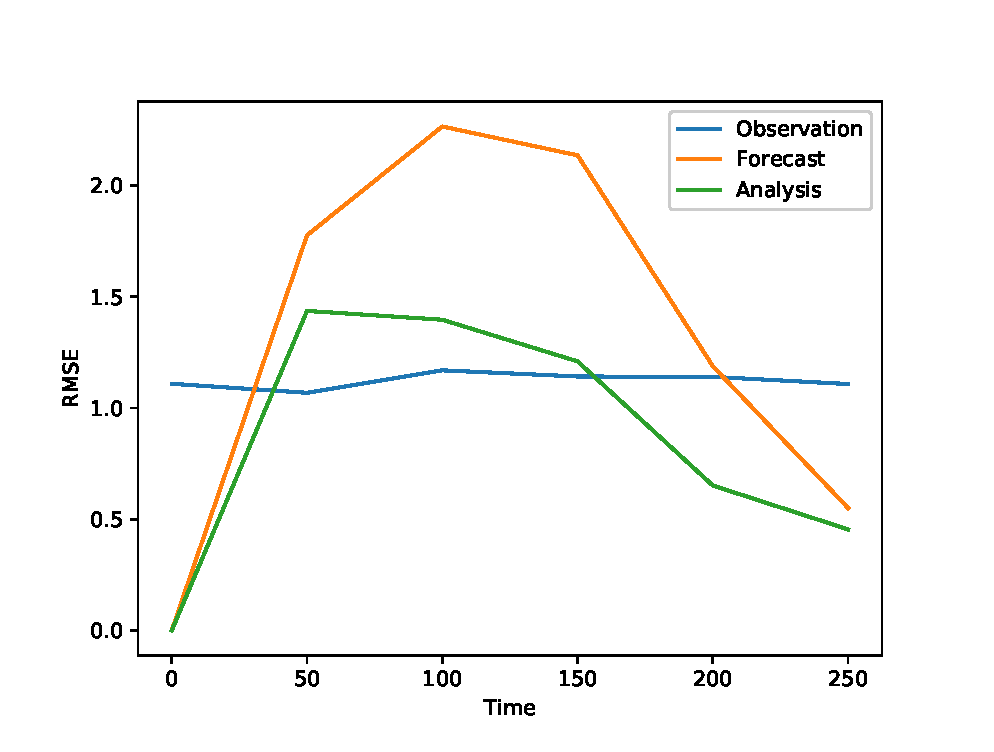
\includegraphics[width=\textwidth]{rmse_comparison.eps}
    \caption[Comparison of errors in model forecasts, model analysis and
    observations at each assimilation point.]{\centering Comparison of errors in
    model forecasts, model analysis and observations at each assimilation point;
    Root Mean Square Error (RMSE) is calculated relative to the ground truth
    with averaging performed over all agents.}\label{fig:rmse_comparison}
\end{figure}

Given that each of the realisations in the ensemble are initialised by taking a
deep-copy of the base-model used to produce truth data, both the forecast and
analysis errors at $k=0$ are $0$.
As model-time passes, the agents enter the model environment, interacting as
their paths cross.
These interactions inject some stochasticity into the model, and consequently
the error in the forecast grows; at $k=50$, we observe that $RMSE_{50}^{f}
\approx 1.75$.
The updating of the model state based on the observations at $k=50$ results in a
reduction in the model error to $RMSE_{50}^{a} \approx 1.4$ confirming, as in
Sections \ref{sec:results:model} and \ref{sec:results:agent}, that the data
assimilation scheme is effective in reducing model error.

The application of the Ensemble Kalman Filter at subsequent assimilation steps
continues to reduce the model error, with greater reductions being observed at
$k=100$ and $k=150$.
It is noteworthy that at $k=150$, where $RMSE_{150}^{f} > 2$ (i.e. over twice
the error in the observations), the observations perform only marginally better
than the analysis with $RMSE_{150}^{o} = 1.1$ and $RMSE_{150}^{a} = 1.2$.
Beyond this point in model-time, the model analysis outperforms the
observations, with $RMSE_{k}^{a} < RMSE_{k}^{o}$ for $k=200$ and $k=250$.

%\begin{figure}[h]
    %\centering
    %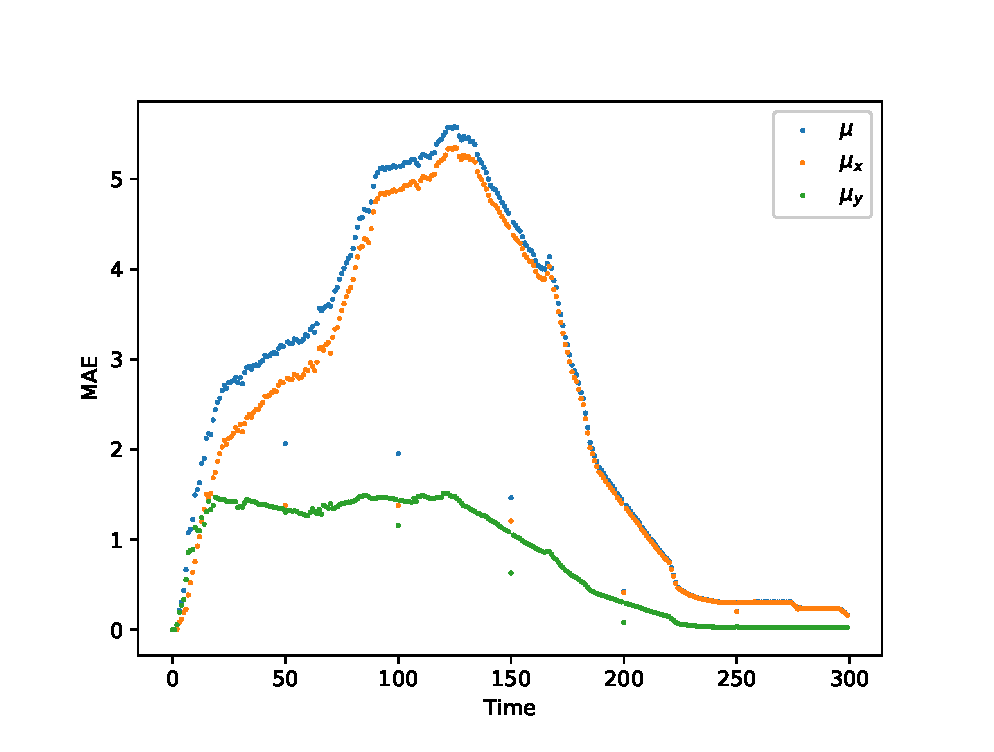
\includegraphics[width=0.8\textwidth]{errors}
    %\caption{Variation of errors with simulation time.}
    %\label{fig:errors}
%\end{figure}
